\section*{Competition, Adaptation and Biodiversity:\\How Fungi Support Our Biosphere}

\setcounter{figure}{0}

Fungi are everywhere in the world, not just on a rotten orange, or in yeast essential bread and cake. Fungi together with a series of other microbes plays an important role in the biosphere, know as the \textbf{decomposers}. The normal functionality of biosphere requires both sustained energy and material flow, and the latter one consists of not only essential organic chemical compound such as amino acids and glucose, but also inorganic carbon dioxide. Such material flow is also called the \textbf{carbon cycle}.

\begin{figure}[ht]
    \centering
    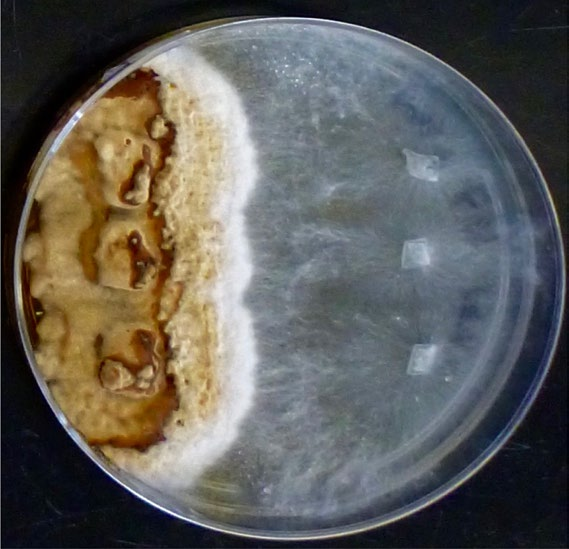
\includegraphics[width=0.4\textwidth]{isolate.jpg}
    \caption{Fungi in pair wise competition test. This figure is adopted from ``Consistent trade-offs in fungal trait expression across broad spatial scales" by Daniel S. Maynard et al.}
    \label{fig:decom-hyphal-122d}
\end{figure}

In carbon cycle, the \textbf{producers}, mainly the green plants, are responsible for the fixation of carbon, namely transforming the carbon in carbon dioxide into fixed carbon in organic matter through chemosynthesis, of which the most commonly known one is photosynthesis. Then, the \textbf{consumers} utilize these material for vital activities, some carbon transformed into again into the carbon dioxide, some maintain in consumers.

What would these carbon go? Can they go back to the atmosphere? This is where decomposers play a role. Decomposers decompose the cadavers and excrements, function as the bridge in the carbon cycle. Note that, one of the most important features of carbon cycle is that it was global, the beef, egg and milk consumptions in the US might be related to the depletion of Brazilian rain forests, which is why carbon cycle is significant to us all and more and more researchers are interested in this topic.

As an important category in decomposers, fungi are outstanding participants in the decay process, especially when dealing with ground litter and woody fibers. A recent research presented the mechanism of decay efficiency for fungi community. The decay ability is positively related to the hyphal extension rate and moisture tolerance of a fungus isolate. However, as for a fungi community, the thing is getting more complicated.

\begin{figure}
    \begin{minipage}{0.5\textwidth}
        \centering
        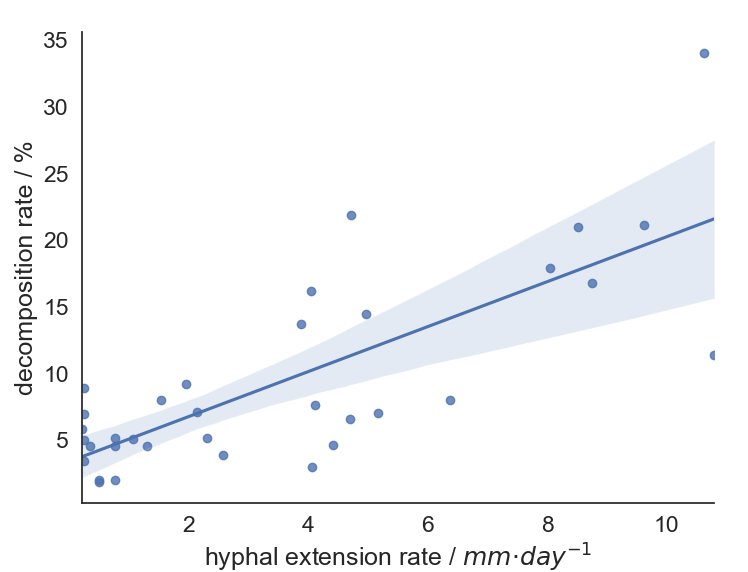
\includegraphics[width=\textwidth]{decom-hyphal-122d.png}
    \end{minipage}
    \begin{minipage}{0.5\textwidth}
        \caption{The relationship between the hyphal extension rate of various fungi and the resulting wood decomposition rate. The hyphal extension rate is the geometrical average of the value tested under 10, 16 and 22 Celsius.}
    \end{minipage}
\end{figure}

The composition of the fungi community can be predicted by the famous Lotka-Volterra model as shown in \eqref{eq:lv}, which indicates that in a multi-species system, each species would exert stress on other species. Tilman interprets that, the intrinsic mechanism is the limitation of certain resources. Generally, the fungus which grows slower, can better tolerate a wide range of environmental conditions. Therefore, some most competitive fungi may attain huge superiority at the start, and replace the less combative fungi completely. Sometime, more tolerant fungi might be able to endure the oppression and gain dominance in the later stages. Such feature determines that, some combinations of fungi may be able to persist and reach a dynamic homeostasis. It is apparent that, these combinations may vary with environmental conditions, you may do your own experiments in the laboratory to find out the ``recipe".

\[
    \label{eq:lv}\tag{$\ast$}
    \frac{\mathrm{d}x_i}{\mathrm{d}t} =
    r_ix_i\left(1 - \frac{\sum_{j=1}^n \alpha_{ij}x_j}{K_i}\right)
\]

Another interesting fact is that, when less competitive species of fungi are introduced to the community, the decay ability of the fungi community may be boosted instead of decreased. This phenomenon can be explained as, different species are preponderant in decomposing at different stages. A large varieties of species, namely the \textbf{biodiversity}, enables the possibility of various combinations. Such combination is relevant to the climatic conditions, resulting unique biodiversity in different geographical areas. Biodiversity also makes the community more variability in face of the variability in local environment.

The global carbon cycle integrates whole biosphere all together, with inconspicuous fungi as a crucial part in it. It is our shared responsibility to restrict carbon emission and protect biodiversity. Biodiversity provides efficiency and robustness to our biosphere. Hope next time you could feel less disgusted when seeing a rotten apple, it might be fungi answering their call!
